\documentclass[a4paper, 12pt, draft]{book}
%\documentclass[a4paper, 12pt, draft]{book}  Nalogo preverite tudi z opcijo draft, ki vam bo pokazala, katere vrstice so predolge!
\usepackage[utf8x]{inputenc}   % omogoča uporabo slovenskih črk kodiranih v formatu UTF-8
\usepackage[slovene,english]{babel}    % naloži, med drugim, slovenske delilne vzorce
\usepackage[pdftex]{graphicx}  % omogoča vlaganje slik različnih formatov
\usepackage{fancyhdr}          % poskrbi, na primer, za glave strani
\usepackage{amssymb}           % dodatni simboli
\usepackage{amsmath}           % eqref, npr.
%\usepackage{hyperxmp}
\usepackage[hyphens]{url}  % dodal Solina
\usepackage{comment}       % dodal Solina
\usepackage{spverbatim}       % dodal Jakob
\usepackage[pdftex, colorlinks=true,
						citecolor=black, filecolor=black, 
						linkcolor=black, urlcolor=black,
						pagebackref=false, 
						pdfproducer={LaTeX}, pdfcreator={LaTeX}, hidelinks]{hyperref}
\usepackage{color}       % dodal Solina
\usepackage{soul}       % dodal Solina
%%%%%%%%%%%%%%%%%%%%%%%%%%%%%%%%%%%%%%%%
%	DIPLOMA INFO
%%%%%%%%%%%%%%%%%%%%%%%%%%%%%%%%%%%%%%%%
\newcommand{\ttitle}{Povezovanje gruč Kubernetes}
\newcommand{\ttitleEn}{Connecting Kubernetes clusters}
\newcommand{\tsubject}{\ttitle}
\newcommand{\tsubjectEn}{\ttitleEn}
\newcommand{\tauthor}{Jakob Hostnik}
\newcommand{\tkeywords}{gruča, oblak, Kubernetes, računalniška gruča, povezovanje gruč, mreža gruč, GitOps}
\newcommand{\tkeywordsEn}{cluster, cloud, Kubernetes, computer cluster, connecting clusters, cluster mesh, GitOps}
%%%%%%%%%%%%%%%%%%%%%%%%%%%%%%%%%%%%%%%%
%	HYPERREF SETUP
%%%%%%%%%%%%%%%%%%%%%%%%%%%%%%%%%%%%%%%%
\hypersetup{pdftitle={\ttitle}}
\hypersetup{pdfsubject=\ttitleEn}
\hypersetup{pdfauthor={\tauthor, jakob@hostnik.si}}
\hypersetup{pdfkeywords=\tkeywordsEn}
%%%%%%%%%%%%%%%%%%%%%%%%%%%%%%%%%%%%%%%%
% postavitev strani
%%%%%%%%%%%%%%%%%%%%%%%%%%%%%%%%%%%%%%%%  
\addtolength{\marginparwidth}{-20pt} % robovi za tisk
\addtolength{\oddsidemargin}{40pt}
\addtolength{\evensidemargin}{-40pt}
\renewcommand{\baselinestretch}{1.3} % ustrezen razmik med vrsticami
\setlength{\headheight}{15pt}        % potreben prostor na vrhu
\renewcommand{\chaptermark}[1]%
{\markboth{\MakeUppercase{\thechapter.\ #1}}{}} \renewcommand{\sectionmark}[1]%
{\markright{\MakeUppercase{\thesection.\ #1}}} \renewcommand{\headrulewidth}{0.5pt} \renewcommand{\footrulewidth}{0pt}
\fancyhf{}
\fancyhead[LE,RO]{\sl \thepage} 
%\fancyhead[LO]{\sl \rightmark} \fancyhead[RE]{\sl \leftmark}
\fancyhead[RE]{\sc \tauthor}              % dodal Solina
\fancyhead[LO]{\sc Diplomska naloga}     % dodal Solina
\newcommand{\BibTeX}{{\sc Bib}\TeX}
%%%%%%%%%%%%%%%%%%%%%%%%%%%%%%%%%%%%%%%%
% naslovi
%%%%%%%%%%%%%%%%%%%%%%%%%%%%%%%%%%%%%%%%  
\newcommand{\autfont}{\Large}
\newcommand{\titfont}{\LARGE\bf}
\newcommand{\clearemptydoublepage}{\newpage{\pagestyle{empty}\cleardoublepage}}
\setcounter{tocdepth}{1}	      % globina kazala
%%%%%%%%%%%%%%%%%%%%%%%%%%%%%%%%%%%%%%%%
% konstrukti
%%%%%%%%%%%%%%%%%%%%%%%%%%%%%%%%%%%%%%%%  
\newtheorem{izrek}{Izrek}[chapter]
\newtheorem{trditev}{Trditev}[izrek]
\newenvironment{dokaz}{\emph{Dokaz.}\ }{\hspace{\fill}{$\Box$}}
%%%%%%%%%%%%%%%%%%%%%%%%%%%%%%%%%%%%%%%%%%%%%%%%%%%%%%%%%%%%%%%%%%%%%%%%%%%%%%%
%% PDF-A
%%%%%%%%%%%%%%%%%%%%%%%%%%%%%%%%%%%%%%%%%%%%%%%%%%%%%%%%%%%%%%%%%%%%%%%%%%%%%%%
%%%%%%%%%%%%%%%%%%%%%%%%%%%%%%%%%%%%%%%% 
% define medatata
%%%%%%%%%%%%%%%%%%%%%%%%%%%%%%%%%%%%%%%% 
\def\Title{\ttitle}
\def\Author{\tauthor, jakob@hostnik.si}
\def\Subject{\ttitleEn}
\def\Keywords{\tkeywordsEn}
%%%%%%%%%%%%%%%%%%%%%%%%%%%%%%%%%%%%%%%% 
% \convertDate converts D:20080419103507+02'00' to 2008-04-19T10:35:07+02:00
%%%%%%%%%%%%%%%%%%%%%%%%%%%%%%%%%%%%%%%% 
\def\convertDate{%
    \getYear
}
{\catcode`\D=12
 \gdef\getYear D:#1#2#3#4{\edef\xYear{#1#2#3#4}\getMonth}
}
\def\getMonth#1#2{\edef\xMonth{#1#2}\getDay}
\def\getDay#1#2{\edef\xDay{#1#2}\getHour}
\def\getHour#1#2{\edef\xHour{#1#2}\getMin}
\def\getMin#1#2{\edef\xMin{#1#2}\getSec}
\def\getSec#1#2{\edef\xSec{#1#2}\getTZh}
\def\getTZh +#1#2{\edef\xTZh{#1#2}\getTZm}
\def\getTZm '#1#2'{%
    \edef\xTZm{#1#2}%
    \edef\convDate{\xYear-\xMonth-\xDay T\xHour:\xMin:\xSec+\xTZh:\xTZm}%
}
\expandafter\convertDate\pdfcreationdate 
%%%%%%%%%%%%%%%%%%%%%%%%%%%%%%%%%%%%%%%%
% get pdftex version string
%%%%%%%%%%%%%%%%%%%%%%%%%%%%%%%%%%%%%%%% 
\newcount\countA
\countA=\pdftexversion
\advance \countA by -100
\def\pdftexVersionStr{pdfTeX-1.\the\countA.\pdftexrevision}
%%%%%%%%%%%%%%%%%%%%%%%%%%%%%%%%%%%%%%%%
% XMP data
%%%%%%%%%%%%%%%%%%%%%%%%%%%%%%%%%%%%%%%%  
\usepackage{xmpincl}
\includexmp{pdfa-1b}
%%%%%%%%%%%%%%%%%%%%%%%%%%%%%%%%%%%%%%%%
% pdfInfo
%%%%%%%%%%%%%%%%%%%%%%%%%%%%%%%%%%%%%%%%  
\pdfinfo{%
    /Title    (\ttitle)
    /Author   (\tauthor, jakob@hostnik.si)
    /Subject  (\ttitleEn)
    /Keywords (\tkeywordsEn)
    /ModDate  (\pdfcreationdate)
    /Trapped  /False
}
%%%%%%%%%%%%%%%%%%%%%%%%%%%%%%%%%%%%%%%%%%%%%%%%%%%%%%%%%%%%%%%%%%%%%%%%%%%%%%%
%%%%%%%%%%%%%%%%%%%%%%%%%%%%%%%%%%%%%%%%%%%%%%%%%%%%%%%%%%%%%%%%%%%%%%%%%%%%%%%
\begin{document}
\selectlanguage{slovene}
\frontmatter
\setcounter{page}{1} %
\renewcommand{\thepage}{}       % preprecimo težave s številkami strani v kazalu
\newcommand{\sn}[1]{"`#1"'}                    % dodal Solina (slovenski narekovaji)
%%%%%%%%%%%%%%%%%%%%%%%%%%%%%%%%%%%%%%%%
%naslovnica
 \thispagestyle{empty}%
   \begin{center}
    {\large\sc Univerza v Ljubljani\\%
      Fakulteta za računalništvo in informatiko\\%
      Fakulteta za matematiko in fiziko}%
    \vskip 10em%
    {\autfont \tauthor\par}%
    {\titfont \ttitle \par}%
    {\vskip 3em \textsc{DIPLOMSKO DELO\\[5mm]        
    INTERDISCIPLINARNI UNIVERZITETNI\\ ŠTUDIJSKI PROGRAM PRVE STOPNJE\\ RAČUNALNIŠTVO IN MATEMATIKA}\par}%
    \vfill\null%
    {\large \textsc{Mentor}: izr. prof. dr. Mojca Ciglarič \par}%
   {\large \textsc{Somentor}:  asist. dr. Matjaž Pančur \par}%
    {\vskip 2em \large Ljubljana, 2021 \par}%
\end{center}
% prazna stran
%\clearemptydoublepage      % dodal Solina (izjava o licencah itd. se izpiše na hrbtni strani naslovnice)
%%%%%%%%%%%%%%%%%%%%%%%%%%%%%%%%%%%%%%%%
%copyright stran
\thispagestyle{empty}
\vspace*{8cm}
\noindent
{\sc Copyright}. 
Rezultati diplomske naloge so intelektualna lastnina avtorja in Fakultete za računalništvo in informatiko Univerze v Ljubljani.
Za objavo in koriščenje rezultatov diplomske naloge je potrebno pisno privoljenje avtorja, Fakultete za računalništvo in informatiko ter mentorja.
\begin{center}
\mbox{}\vfill
\emph{Besedilo je oblikovano z urejevalnikom besedil \LaTeX.}
\end{center}
% prazna stran
\clearemptydoublepage
%%%%%%%%%%%%%%%%%%%%%%%%%%%%%%%%%%%%%%%%
% stran 3 med uvodnimi listi
\thispagestyle{empty}
\vspace*{4cm}
\noindent
Fakulteta za računalništvo in informatiko izdaja naslednjo nalogo:
\medskip
\begin{tabbing}
\hspace{32mm}\= \hspace{6cm} \= \kill
Tematika naloge:
\end{tabbing}
Preučite področje povezovanja gruč Kubernetes. Analizirajte problematiko povezovanja in preglejte nekaj primerov uporabe, ki izvirajo iz potreb podjetij. Pripravite tudi prototipno rešitev povezovanja, pri čemer se osredotočite na rešitve, nastale v odprtokodni skupnosti Kubernetes.
\vspace{15mm}
\vspace{2cm}
% prazna stran
\clearemptydoublepage
% zahvala
\thispagestyle{empty}\mbox{}\vfill\null\it%
\noindent
Na tem mestu bi se zahvalil mentorici izr. prof. dr. Mojci Ciglarič in somentorju asist. dr. Matjažu Pančurju za pripravljenost, mentorstvo, vse nasvete in pomoč pri pisanju diplomske naloge.
Zahvala pa gre tudi moji ženi, staršem, bratom, sestram in prijateljem za podporo in spodbudo pri študiju.
\rm\normalfont
% prazna stran
\clearemptydoublepage
%%%%%%%%%%%%%%%%%%%%%%%%%%%%%%%%%%%%%%%%
% posvetilo, če sama zahvala ne zadošča :-)
\thispagestyle{empty}\mbox{}{\vskip0.20\textheight}\mbox{}\hfill\begin{minipage}{0.55\textwidth}%
Mami Lučki.
\normalfont\end{minipage}
% prazna stran
\clearemptydoublepage
%%%%%%%%%%%%%%%%%%%%%%%%%%%%%%%%%%%%%%%%
% kazalo
\pagestyle{empty}
\def\thepage{}% preprecimo tezave s stevilkami strani v kazalu
\tableofcontents{}
% prazna stran
\clearemptydoublepage
%%%%%%%%%%%%%%%%%%%%%%%%%%%%%%%%%%%%%%%%
% seznam kratic
\chapter*{Seznam uporabljenih kratic}  % spremenil Solina, da predolge vrstice ne gredo preko desnega roba
\noindent\begin{tabular}{p{0.15\textwidth}|p{.375\textwidth}|p{.375\textwidth}}    % po potrebi razširi prvo kolono tabele na račun drugih dveh!
  {\bf kratica} & {\bf angleško}                             & {\bf slovensko} \\ \hline
  {\bf CRD} & custom resource definition & definicija tipov po meri \\
  {\bf DNS} & domain name system & sistem domenskih imen \\
  {\bf IP} & internet protocol & internetni protokol \\
  {\bf HA} & high availability & visoka razpoložljivost \\
  {\bf GA} & general availability & splošna dostopnost \\
  {\bf VPN} & virtual private network & navidezno zasebno omrežje \\
  {\bf TOSCA} & topology and orchestration specification for cloud applications & specifikacija topologije in orkestracije za aplikacije v oblaku \\
  {\bf WAN} & wide area network & prostrano omrežje \\
\end{tabular}
% prazna stran
\clearemptydoublepage
%%%%%%%%%%%%%%%%%%%%%%%%%%%%%%%%%%%%%%%%
% povzetek
\addcontentsline{toc}{chapter}{Povzetek}
\chapter*{Povzetek}
\noindent\textbf{Naslov:} \ttitle
\bigskip

\noindent\textbf{Avtor:} \tauthor
\bigskip
%\noindent\textbf{Povzetek:} 
\noindent 

Ko na strežnikih začne zmanjkovati virov, obstajata dva standardna na\-či\-na za povečanje virov v našem sistemu.
Prva možnost je, da strežnike nadgradimo, druga pa, da jih kupimo več in jih povežemo v računalniško gručo.
V zadnjih letih se je na tem področju zgodil preboj s pojavom sistema Kubernetes.
Sistem je zaradi svoje popularnosti postal \emph{de facto} standard za upravljanje gruč in orkestracijo kontejnerjev.
A ena sama gruča ni vedno dovolj v primerih, ko imamo težave z dragim prenosom podatkov, preveliko latenco do naših uporabnikov ali pa, ko želimo še bolj povečati stabilnost ali varnost našega sistema.
Predstavili bomo ozadje povezovanja gruč in pristope, ki jih lahko uporabimo za reševanje naših problemov.
Poseben poudarek bomo dali tudi na sinhronizacijo podatkov, saj je to eden zahtevnejših delov pri upravljanju več računalniških gruč.
Ugotavljamo, da nam lahko predstavljene sodobne metode povezovanja gruč zelo olajšajo njihovo upravljanje in preprosto rešijo tudi zahtevnejše probleme sinhronizacije podatkov.

\bigskip
\noindent\textbf{Ključne besede:} \tkeywords.
% prazna stran
\clearemptydoublepage
%%%%%%%%%%%%%%%%%%%%%%%%%%%%%%%%%%%%%%%%
% abstract
\selectlanguage{english}
\addcontentsline{toc}{chapter}{Abstract}
\chapter*{Abstract}
\noindent\textbf{Title:} \ttitleEn
\bigskip

\noindent\textbf{Author:} \tauthor
\bigskip
%\noindent\textbf{Abstract:} 
\noindent 

When we are running low on resources in our computer system, there are two standard solutions for increasing them.
The first solution is to upgrade our servers and the second one is to buy more servers and connect them to a cluster.
There has been a major breakthrough in this field with the release of the Kubernetes system in recent years.
The system became de facto standard for cluster management and container orchestration.
But when we have problems such as expensive data transfer, too much latency to our users, or we want to further increase the stability or security of our system one cluster is not always enough.
We will look at the background of connecting clusters and what approaches we can use to solve our problems.
Furthermore, we will also place special emphasis on data synchronization, as this is one of the more difficult parts of managing multiple computer clusters.
We find that presented modern methods of connecting clusters can greatly facilitate their management and easily solve even more difficult data synchronization problems.

\bigskip
\noindent\textbf{Keywords:} \tkeywordsEn.
\selectlanguage{slovene}
% prazna stran
\clearemptydoublepage
%%%%%%%%%%%%%%%%%%%%%%%%%%%%%%%%%%%%%%%%
\mainmatter
\setcounter{page}{1}
\pagestyle{fancy}
\chapter{Uvod}
\label{uvod}
\section{Motivacija}
Leta 2014 je Google objavil kodo sistema za orkestracijo kontejnerjev Kubernetes~\cite{what-is-Kubernetes}~\cite{borg-omega-kubernetes}.
Kubernetes  je univerzalni način, ki omogoča, da več ra\-ču\-nal\-ni\-kov povežemo v gručo, ki deluje kot samostojna enota. 
Povezovanje strežnikov v gruče omogoča visoko razpoložljivost (HA) naših storitev~\cite{mastering-kubernetes}, deljenje virov in preprostejšo sinhronizacijo podatkov.
V primerih, obravnavanih v tem delu, pa ni dovolj uporaba ene same gruče, ampak moramo med seboj povezati in upravljati več gruč.
V zadnjem času so razvijalci Kubernetesa začeli bolj celostno reševati ta problem.
Poskusili so ga rešiti s projektom Federation 1, po njegovi ukinitvi~\cite{kubernetes-federation-evolution} pa razvijalci Federation 2 oziroma KubeFed trdijo, da bo projekt uspešno prešel iz alfa v beta verzijo~\cite{kubefed-repo}.
\section{Cilj in vsebina naloge}
V diplomskem delu bomo obravnavali rešitve problema povezovanja gruč Kubernetes in primere uporabe, ki izvirajo iz potreb industrije.
Vsakemu primeru bomo poiskali rešitev v okolju Kubernetes z uporabo orodja KubeFed, poudarek pa bomo dali na sinhronizacijo podatkov.
\subsection{Prevelika latenca}
Problem prevelike latence se pojavi, ko je čas od poslanega zahtevka uporabnika do prejema odgovora s strežnika prevelik~\cite{minimizing-latency}.
Ko problem povzroča velika fizična razdalja, ga rešimo tako, da postavimo dodatne gruče bližje naših uporabnikov, denimo na njihovo celino.
Zavedati se moramo, da strežniki v gruči zelo veliko komunicirajo, zato je priporočljivo, da se nahajajo v istem omrežju znotraj istega podatkovnega centra, saj se s tem izognemo veliki latenci ~\cite{kube-and-edge}.
\begin{figure}[h]
\begin{center}
  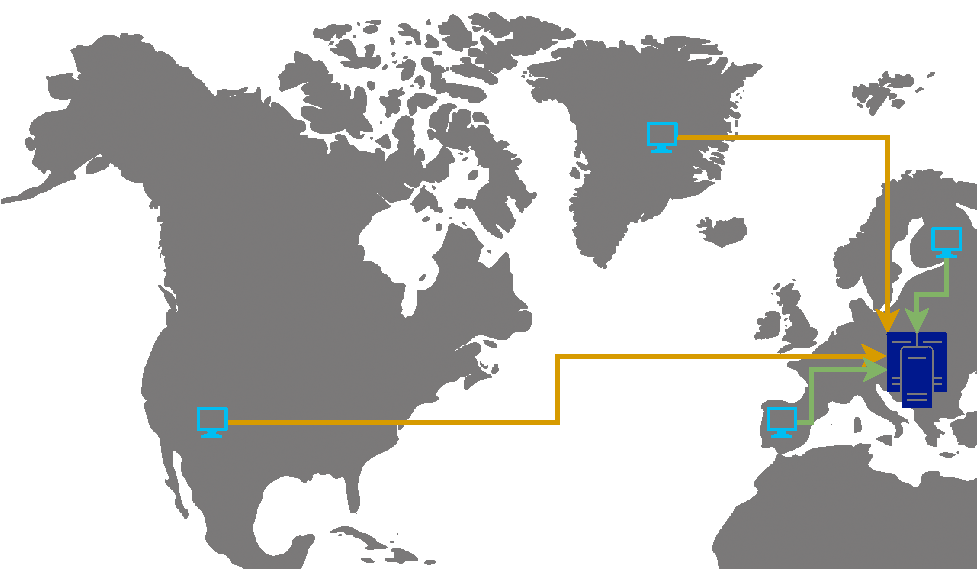
\includegraphics[width=1.0\textwidth]{images/problem-prevelike-latence.pdf}
\end{center}
\caption{Problem prevelike latence.}
\label{problem-prevelike-latence}
\end{figure}
\subsection{Visoka razpoložljivost}
Večkrat letno pride do izpada kakšnega večjega podatkovnega centra~\cite{ha-systems}. 
To se lahko zgodi iz več razlogov najpogosteje pa gre za napake na programski opremi ~\cite{common-outages}.
Če gre v takšnem primeru za oblačnega ponudnika, pri katerem imamo nameščeno svojo gručo, to pomeni, da bo hkrati nedosegljiva tudi ta.
V splošnem se problem reši tako, da uporabljamo več gruč in jih namestimo v več različnih podatkovnih centrov.
V primeru izpada enega podatkovnega centra pa svoje uporabnike preusmerimo v drug podatkovni center.
\subsection{Potreba po izolaciji aplikacij}
Ko govorimo o izolaciji aplikacije, se navezujemo na varnost pri vdoru ali pa na večjo razpoložljivost.
Uporaba Kubernetesa od nas zahteva izolacijo v kontejnerje.
Prav tako pa nam že sam Kubernetes omogoča izolacijo na posamezne strežnike~\cite{kube-network-policy} ali nastavitev pravil komunikacije v gruči~\cite{kube-pod-to-node}.
Kljub tem postopkom se v Kubernetesu pojavljajo problemi, zaradi katerih postane nedosegljiva celotna gruča, s tem pa vse aplikacije v tej gruči.
Če postavimo del neodvisnih aplikacij v drugo gručo, s tem preprečimo njihov izpad ob napaki v prvi gruči.
Izolacija pa je pomembna tudi z varnostnega vidika.
Če se napadalec polasti enega samega vozlišča, ima posledično tudi popolno kontrolo nad vsemi drugimi aplikacijami, ki tečejo na tem vozlišču~\cite{securing-kube}.
Aplikacije lahko pripadajo istemu uporabniku ali pa celo drugim uporabnikom.
Če imamo vsako aplikacijo v svoji gruči, pa se temu lahko izognemo.
\chapter{Problem povezovanja gruč}
Računalniška gruča je skupina računalnikov, ki zaradi večje zanesljivosti in zmogljivosti opravlja določene storitve.

Zaradi prevelike latence ali drugih ovir računalnikov ne moremo povezati v eno tesno povezano gručo~\cite{kube-and-edge}.
Računalnike lahko vedno povežemo v več različnih gruč, četudi to pomeni, da je v nekaterih gručah samo po en strežnik oziroma vozlišče.
Ob prisotnosti povezave pa lahko te gruče med seboj povežemo, a šibkeje.

Ko govorimo o tesni povezanosti znotraj gruče, velja, da ima vsako vozlišče dostop do vsakega, da vsak kontejner lahko komunicira z vsakim in da so vozlišča v istem hitrem notranjem omrežju podatkovnega centra. 
Pričakujemo, da sistem, ki ga uporabljamo za gručenje, omogoča razporejanje zaželenih storitev in kontejnerjev med strežniki in v primeru izpada vozlišča to odstrani iz sistema, kontejnerje s tega vozlišča pa prerazporedi na preostala vozlišča.

Šibka povezanost med gručami pomeni, da je povezava med različnimi gručami počasna, nezanesljiva ali draga.
Zaradi omejitev moramo sprejemati kompromise na podlagi zmožnosti povezave.
Skladno z našimi potrebami se lahko odrečemo komunikaciji med vozlišči v različnih gručah.
Pričakujemo, da vsaka gruča skrbi za svoja vozlišča ter svoje storitve in kontejnerje ohranja v delovanju.
V tem delu bomo kot naloge sistemov za povezovanje gruč obravnavali: omogočanje centralnega nadzora nad storitvami v gručah, prerazporejanje teh storitev med gručami, dinamično odkrivanje drugih gruč in njihovih storitev, izločanje nedosegljivih gruč, povezljivost med vsemi vozlišči in kontejnerji, četudi so vozlišča v različnih omrežjih.

\begin{figure}[h]
\begin{center}
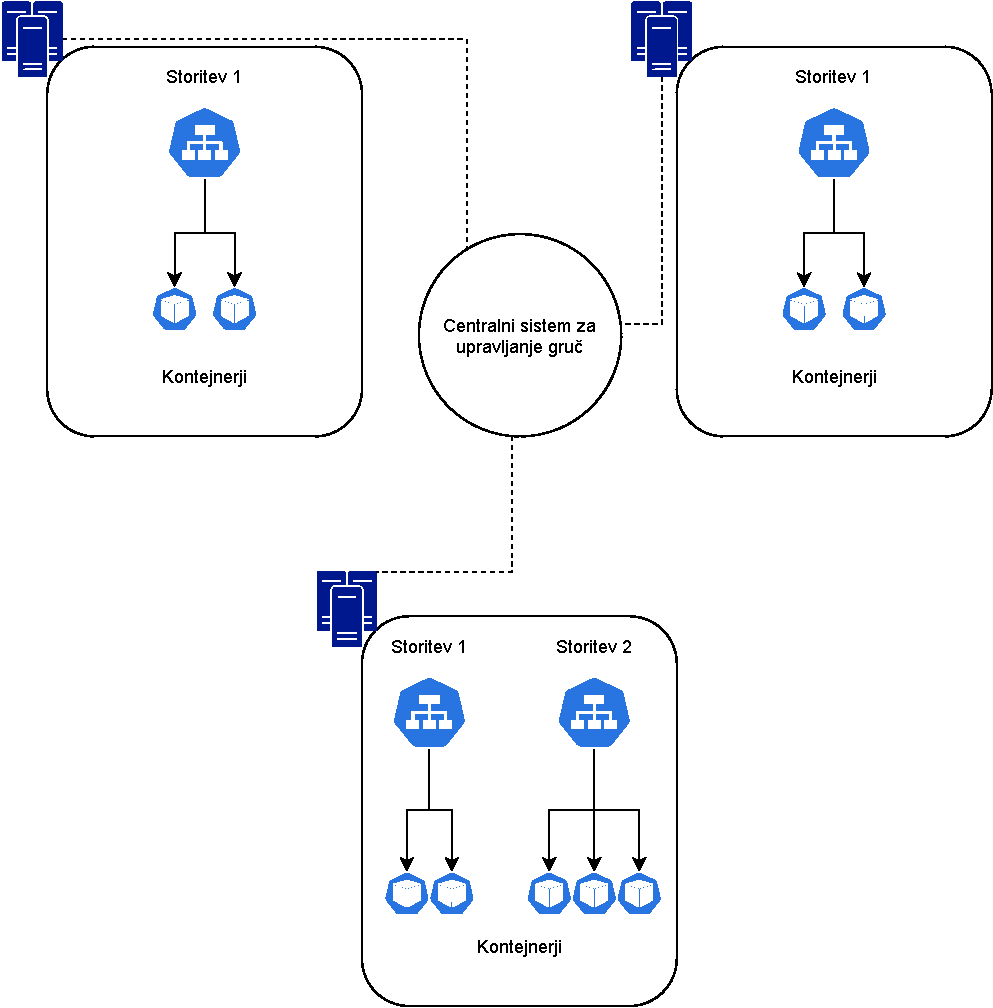
\includegraphics[width=1.0\textwidth]{images/primer-povezanih-gruc.pdf}
\end{center}
\caption{Primer več povezanih gruč.}
\label{problem-povezanih-gruc}
\end{figure}

\chapter{Kubernetes}
\label{Kubernetes}
Kubernetes definira javno dostopen vmesnik REST.
Trenutno obstaja že več kot 70 distribucij~\cite{cncf} Kubernetesa.
\section{Zgodovina}
Leta 2014 je Google objavil in odprl kodo projekta Kubernetes~\cite{mastering-kubernetes}~\cite{borg-omega-kubernetes}.
Gre za program, ki je bil ustvarjen z namenom, da poenostavi upravljanje kontejnerjev in večjih računalniških gruč v produkcijskih okoljih~\cite{what-is-Kubernetes}.
A to niso pravi začetki Kubernetesa.
Začelo se je leta 2003, ko je Google začel z razvojem sistema za upravljanje svojih notranjih gruč Borg.
Pozneje, leta 2013, je Google predstavil sistem Omega, leta 2014 pa je objavil odprtokodni projekt Kubernetes. 
Projekt je bil zasnovan na podlagi dobrih praks upravljanja s kontejnerji, ki so se jih pri Googlu naučili skozi dolga leta upravljanja velikega števila kontejnerjev v produkcijskem okolju.
Pozneje je upravljanje nad projektom prevzela organizacija Cloud Native Computing Fundation.
\section{Osnovni pojmi}
Kubernetesov vmesnik REST nam omogoča, da v sistem shranjujemo najrazličnejše tipe objektov.
Takšne, ki so del standardnega Kubernetesovega vmesnika, ali pa smo jih definirali sami (CRD).
Najpogostejši tipi objektov, ki se pojavijo v Kubernetesu so Pod, Service, Deployment, StatefulSet in objekti za delo z diski.
\begin{figure}[h]
\begin{center}
\includegraphics[width=1.0\textwidth]{images/Kubernetes-simple-schema.pdf}
\end{center}
\caption{Primer delovanja objektov Kubernetes.}
\label{problem-povezanih-clustrov}
\end{figure}
\subsection{Pod}
Objekt Pod je najmanjša enota v Kubernetesu, ki lahko teče v gruči~\cite{pod}.
Sestavljen je iz enega ali več kontejnerjev, ki si delijo diske in omrežni vmesnik.
To pomeni, da imajo skupen naslov IP in se obnašajo podobno kot izolirani procesi na istem računalniku.
\subsection{Service}
Objekt Service označuje vse objekte Pod ene storitve~\cite{service}.
Kubernetes iz objekta v notranjem DNS ustvari domeno za storitev in dinamično porazdeljuje promet med našimi objekti Pod.
Objekte Service uporabljamo tako, da namesto pošiljanja zahtevkov neposredno na naslov IP objekta Pod, zahtevke pošiljamo na ustvarjeno domensko ime storitve na primer \spverb|curl ime-storitve|.
Takšen zahtevek nato dobi eden izmed označenih objektov Pod v objektu Service.
\subsection{Deployment}
Deployment je objekt, ki mu podamo število želenih objektov Pod in predlogo za njihovo izdelavo~\cite{deployment}.
Notranje storitve Kubernetesa nato zagotavljajo, da bo obstajalo toliko takšnih objektov tipa Pod, kot smo navedli v definiciji objekta Deployment.
Takšno stanje se poskuša ohranjati tudi ob raznih težavah in izpadih vozlišč.
\subsection{StatefulSet}
Ta objekt je zelo podoben objektu Deployment, le da StatefulSet vsakemu objektu Pod dodeli unikatno številko~\cite{statefulset}. 
Pod, ki se ustvari s to številko, ohranja diske, mrežni vmesnik, naslov IP in domensko ime.
Pomembna razlika med objektoma Deployment in StatefulSet pa je tudi v polju \spverb|volumeClaimTemplate|.
StatefulSet omogoča vsakemu objektu Pod, da ustvari in uporablja svoj disk.
Uporablja pa se za podatkovne baze in podobne storitve, ki morajo ohranjati stanja.
\chapter{Pregled področja in literature}
V tem poglavju bomo predstavili nekaj ključnih del in literature s področja povezovanja gruč Kubernetes.
V delih sta pogosto za federacijo izbrana sistema Federation 1 ali Federation 2 zaradi tesne povezanosti s sistemom Kubernetes~\cite{tosca-fed}~\cite{dyn-place}~\cite{kube-and-edge}.

V članku \cite{tosca-fed} se avtorji lotijo povezovanja gruč pri različnih oblačnih ponudnikih.
Pri tem pozornost namenijo tudi avtomatskemu horizontalnemu skaliranju aplikacij.
Za uporabo in postavitev pri več oblačnih ponudnikih so uporabili standard TOSCA, ki jim omogoča enoten deklarativni zapis njihove strukture v različnih oblakih.
V svoji študiji so uporabili sistem Cloudify, ki pa jim z dodatkom za Kubernetes omogoča tudi enoten način namestitve Kubernetesa.
Svoje gruče so povezali v federacijo s sistemom Federation. 
Iz članka pa ni povsem razvidno ali so uporabili prvo ali drugo iteracijo tega sistema.
V testne namene so v federacijo namestili še strežnik spletne igre in pokazali uspešnost avtomatskega horizontalnega skaliranja.

Lorenzo Martino je v magistrski nalogi ~\cite{dyn-place} v uvodu pojasnil pomembnost pristopa mikrostoritev pri razvoju aplikacij in pokazal prednosti uporabe Kubernetesa v oblaku.
Kot glavno prednost je izpostavil neodvisnost od platforme in možnost uporabe sistema Kubernetes v oblaku ali pa v lokalnem podatkovnem centru.
Omenil je tudi hibridne rešitve, ki pa zahtevajo povezovanje in upravljanje več gruč.

V nadaljevanju je podanih nekaj predlogov za uporabo več gruč Kubernetes, kot so: izolacija med produkcijskim in testnim okoljem, težave z latenco zaradi prevelikih fizičnih razdalj, povečevanje razpoložljivosti aplikacije, uporaba dodatne gruče v oblaku zaradi lažjega avtomatskega skaliranja vozlišč, omejitve lokacije obdelovanja podatkov.
V delu je predlaganih tudi nekaj programov za upravljanje gruč, v rešitvi problema pa je avtor uporabil sistem KubeFed.
Avtor omeni, da je pri svojem delu reševal problem v podjetju, ki se ukvarja s civilnimi in vojaškimi aeronavtičnimi sistemi.
Ključna zahteva v podjetju je bila obdelava podatkov v lokalnih gručah.
Nadaljevanje dela je vezano na reševanje konkretnega problema podjetja.
V delu je posebna pozornost namenjena sinhronizaciji podatkov, saj imajo v podjetju označene podatke, ki se ne smejo obdelovati v oblaku, in podatke, ki se lahko.
KubeFed je še v razvojni fazi alfa, kar pa je za podjetje predstavljalo oviro.
Tako je avtor poleg rešitve s KubeFed pripravil še svojo rešitev, v kateri implementira samo potrebne funkcionalnosti.

Vir ~\cite{kube-and-edge} pa se posveti področju upravljanja aplikacij na robu oblaka, kjer pride centralno upravljanje zaradi večjega števila gruč še bolj do izraza.
V poročilu je gruča Kubernetes postavljena v prostrano omrežje (WAN).
Avtorji so primerjali delovanje ene gruče preko prostranega omrežja z delovanjem iste gruče preko lokalnega omrežja.
Pri takšnem pristopu v gručah na robu oblaka izpostavijo pomembnost previdnosti, saj lahko pride do nepredvidljivih rezultatov.
V poročilu je predstavljen tudi odprtokodni sistem KubeEdge.
Projekt je namenjen razširitvi aplikacij v kontejnerjih na vozlišča na robu oblaka~\cite{kubeedge}.
Avtorji izpostavijo, da imata tako pristop z eno gručo v omrežju WAN kot pristop s sistemom KubeEdge pomembno omejitev, saj imajo vozlišča v primeru izpada iz omrežja še vedno premalo avtonomnosti.
Izpostavljeno je, da te slabosti rešimo s federacijo in sistemom KubeFed, ki je v nadaljevanju podrobneje opisan.
Če je vsako vozlišče v svoji gruči, potem je vozlišče v primeru izpada omrežja še vedno avtonomno in omogoča lokalno upravljanje.

\chapter{Povezovanje gruč Kubernetes}
Ko postavimo več različnih gruč, imamo vedno možnost, da upravljamo vsako posebej.
Toda takšen pristop ni učinkovit, če imamo takšnih gruč res veliko~\cite{difference-multi-cluster}.
Osnovna lastnost sistema za upravljanje več gruč Kubernetes je možnost prenašanja Kubernetesovih objektov med gručami.
Tako lahko objekt definiramo samo enkrat in naš sistem ga bo ustvaril v izbranih gručah.
Glede na potrebe pa lahko uporabimo sistem, ki omogoča tudi dinamično odkrivanje storitev z enako definicijo v različnih gručah, komunikacijo med storitvami v različnih gručah, dinamično odkrivanje objektov Pod med gručami in komunikacijo med njimi v različnih gručah.
Te funkcionalnosti znotraj ene gruče nudi že Kubernetes.
Od našega primera pa je odvisno, katere funkcionalnosti želimo uporabiti in kako kompleksno postavitev potrebujemo.
V nadaljevanju bomo predstavili različne sisteme za povezovanje gruč Kubernetes, njihove glavne prednosti in značilnosti.
\section{ArgoCD in drugi sistemi GitOps}
\subsection{Sinhronizacija objektov z uporabo sistemov GitOps}
Osnovna ideja pristopa GitOps je, da imamo strukturo aplikacij v gruči Kubernetes napisano v repozitoriju Git in potem je kontroler GitOps tisti, ki iz teh definicij postavi strukturo gruče.
Takšen pristop se je v zadnjih letih zelo razširil in ArgoCD navaja več kot sto podjetij, ki ga uporabljajo pri razvoju~\cite{argocd-user-list}.

Če uporabljamo kakšnega od sistemov GitOps, lahko iz enakega repozitorija postavimo več gruč.
V osnovi takšen pristop omogoča, da bomo imeli na voljo samo sinhronizacijo infrastrukture in nam ne omogoča naprednih funkcionalnosti, kot so komunikacija med objekti Pod v različnih gručah ali pa odkrivanje storitev ali kontejnerjev.
V nadaljevanju bomo izbrali sistem ArgoCD in pogledali, kako bi postavili zgoraj opisano infrastrukturo.
\subsection{Sinhronizacija objektov z ArgoCD}
ArgoCD podpira več različnih formatov konfiguracije gruče~\cite{argocd-docs}.
Uporabimo lahko format datoteke YAML z definicijami objektov, ki jih želimo namestiti v vsako gručo.
Za nameščanje te konfiguracije v več kot eno gručo imamo na voljo dva pristopa.
Prvi je, da v vsako gručo namestimo ArgoCD in uporabimo enak repozitorij Git v vsaki izmed njih.
ArgoCD pa nam omogoča tudi pošiljanje konfiguracije v oddaljene gruče~\cite{declarative-setup}.
To pomeni, da imamo lahko kontroler ArgoCD nameščen samo v eni gruči.

Če ne želimo, da imajo vse gruče popolnoma enako infrastrukturo in nameravamo prilagoditi konfiguracijo posamezne gruče, lahko uporabimo format zapisa konfiguracije, ki podpira predloge.
ArgoCD nam ponuja možnost, da v predlogah sami določimo vrednosti spremenljivk.
Tako lahko uporabimo na primer predloge Helm in ArgoCD nam bo omogočil, da vsaki gruči izberemo lastno datoteko s spremenljivkami.
Glede na preprostost delovanja takšnega sistema se moramo zavedati, da od njega ne moremo pričakovati nikakršnih naprednih funkcionalnosti kot sta dinamično odkrivanje storitev in komunikacija kontejnerjev med gručami.
Takšen sistem nam omogoča samo sinhronizacijo infrastrukture.

\begin{figure}[h]
\begin{center}
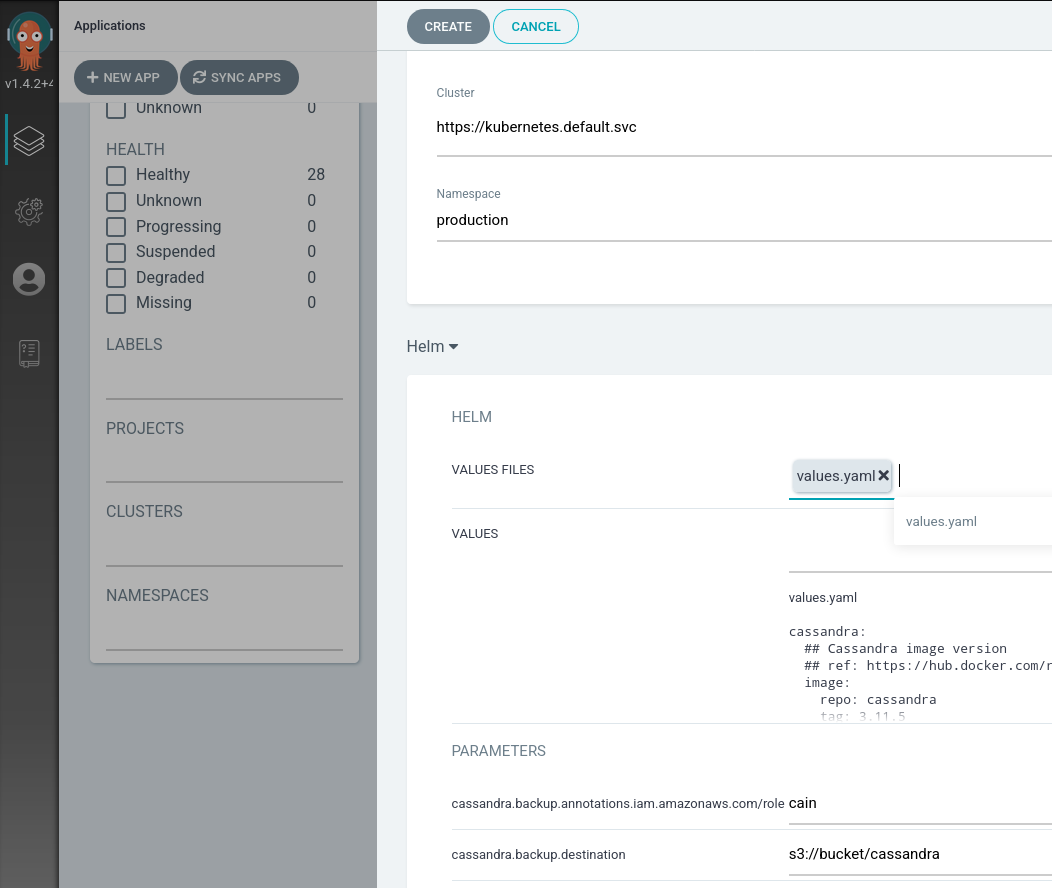
\includegraphics[width=1.0\textwidth]{images/primer-uporabe-helm-predloge-argo-cd.png}
\end{center}
\caption{Primer uporabe predloge Helm v ArgoCD.}
\label{primer-uporabe-helm-predloge-argo-cd}
\end{figure}

\section{KubeFed}
9. 1. 2018 je bil po ukinjenem projektu Kubernetes Federation V1 ustvarjen Kubernetes Federation V2, imenovan tudi KubeFed~\cite{kubernetes-federation-evolution}.
Cilj obeh projektov je bil poenostavljeno upravljanje več gruč in razporejanje Kubernetes objektov.
V projektu Federation V1 je bil ubran pristop, ki je skupino gruč ali federacijo uporabniku predstavil kot novo gručo Kubernetes~\cite{setup-cluster-federation-kubefed-v1}.
Uporabljal je svoj vmesnik, ki pa je bil združljiv s Kubernetesovim, kar je omogočalo tudi uporabo orodja kubectl~\cite{cluster-federation-in-Kubernetes-1.5}.
Objekti, ki jih je federacija podpirala, so bili kompatibilni s standardnimi objekti Kubernetes~\cite{federated-cluster-kubefed-v1}.
Objekte, ki so bili poslani kontrolerju federacije, je Federation V1 nato ustvaril tudi v pripadajočih gručah.
Pristop zaradi mnogih pomanjkljivosti in pomankanja možnosti naprednejših konfiguracij ni uspel pridobiti statusa GA.
Faza GA v Kubernetesu pomeni, da se uporabniki lahko zanašajo na projekt, ga uporabljajo in se bo vsaj do neke mere ohranjala združljivost za nazaj.
Pred dosegom te stopnje naj bi se projekt uporabljalo samo v testne namene.

Tako se je pozneje razvil projekt Federation V2~\cite{kubernetes-federation-evolution}.
Glavna razlika s prvo različico je z uporabniškega stališča v tem, da za federacijo ne poizkuša imitirati Kubernetesovega vmesnika, ampak uporablja obstoječega. 
Federation V2 samo predstavi nove objekte, ki pa so razširitev standardnih, kot na primer FederatedDeployment~\cite{kubefed-userguide}.
Federirane objekte je treba najprej vklopiti z ukazom \spverb|kubefedctl enable|.
\begin{verbatim}
kubefedctl enable deployment
\end{verbatim}
Orodje kubefedctl moramo namestiti na svoj računalnik.
Takšen federiran objekt vsebuje tri glavne lastnosti: definicija predloge primarnega objekta, postavitev v gruče in prepis lastnosti originalnega objekta za posamezne gruče.
Takšen pristop je zelo široko zastavljen in omogoča tudi federacijo objektov CRD.
\begin{verbatim}
apiVersion: types.kubefed.io/v1beta1
kind: FederatedDeployment
spec:
  placement:
    clusterSelector:
      # izbira gruč
      matchLabels: {}
      ... 
  template:
    # specifikacije objekta deployment
    spec:
    ... 
  overrides:
    # prepis konfiguracije za posamezne gruče
    - clusterName: gruca-1
      clusterOverrides:
          # nastavi polje replicas na vrednost 5
        - path: "/spec/replicas"
          value: 3
  ... 
\end{verbatim}
Federation V2 poleg sinhronizacije infrastrukture podpira tudi odkrivanje storitev v drugih gručah prek zapisov DNS~\cite{kubefed-userguide}.
Omenja pa se možnost odstranitve te funkcionalnosti~\cite{remove-service-discovery}, ki je že sedaj privzeto izklopljena.
Preden uporabimo KubeFed pa se moramo zavedati, da je projekt v času pisanja diplomske naloge še vedno v razvojni fazi alfa in lahko preteče še nekaj časa preden doseže status GA.
\section{Cilium}
Cilium je odprtokodni program, ki nam omogoča napredne varnostne in omrežne nastavitve v gruči~\cite{cilium-intro}.
Program na tretji in četrti omrežni plasti zagotavlja osnovne principe varnosti in zaščite, kot sta, na primer, zapiranje portov in omejevanje komunikacije.
Poleg tega pa Cilium zagotavlja tudi naprednejšo varnost na sedmi omrežni plasti, saj omogoča omejevanje in filtriranje zahtevkov HTTP in podobne varnostne funkcionalnosti na popularnih protokolih aplikacijskega nivoja~\cite{cilium-intro}.

Ker Cilium implementira precejšen del mreženja in povezovanja v Kubernetesu, pa nam s tem lahko ponudi tudi nekaj zelo naprednih možnosti, ko med seboj povezujemo več različnih gruč Kubernetes.
Tako nam Cilium kot ključni prednosti omogoča tudi komunikacijo med kontejnerji v različnih gručah~\cite{cilium-cluster-mesh} in uporabo globalnih objektov Service, ki razporejajo promet med različnimi gručami.
Takšne objekte definiramo z anotacijo \spverb|io.cilium/global-service|~\cite{setup-cilium-cluster-mesh}.
Omogoča nam tudi omejevanje povezovanja med gru\-ča\-mi z njihovim objektom \spverb|CiliumNetworkPolicy|~\cite{setup-cilium-cluster-mesh}.
Ko postavljamo mre\-žo gruč, pa se moramo še vedno zavedati, da Cilium ne rešuje problema, če so naše gruče skrite v različnih zasebnih omrežjih.
Ključno pri uporabi Ciliuma za povezovanje gruč je, da so vsa naša vozlišča med seboj dosegljiva.
A četudi so naše gruče v med seboj direktno nedosegljivih zasebnih omrežjih, je problem rešljiv z uporabo sistema VPN, ki omogoča, da vsa vozlišča povežemo v eno navidezno omrežje~\cite{setup-cilium-cluster-mesh}.

Kljub naprednim funkcijam, ki jih Cilium ponuja, pa se moramo zavedati, da se ukvarja samo s povezovanjem gruč na omrežnem nivoju.
Ne omogoča enotnega upravljanja in sinhronizacije objektov med gručami zato moramo objekte sinhronizirati sami.
Ampak so zaradi dovolj široke zasnove Kubernetesovega vmesnika rešitve med seboj kompatibilne.
Torej lahko uporabimo napredno mreženje Ciliuma in objekte sinhroniziramo s pristopom KubeFed ali GitOps.
\chapter{Priprava sistema gruč za testiranje}
\section{Raspberry PI 4}
Za namene testiranja različnih načinov povezovanja gruč Kubernetes moramo najprej postaviti nekaj gruč.
Zaradi preprostosti in nizke cene, predvsem pa, ker se koncepti zaradi tega ne spremenijo, bomo za naša Kubernetes vozlišča uporabili Raspberry PI 4.
Na višjem nivoju gre še vedno za gručo Kubernetes in delo je zelo podobno, če uporabimo nekaj tisoč vozlišč v gruči v oblaku ali pa lokalno gručo z enim vozliščem.
Raspberry PI 4 je majhen (85x56x20mm) in manj zmogljiv računalnik na eni sami plošči~\cite{rpi-tech-spec}.
Ključni prednosti takšnih računalnikov sta velikost in cena.
Na vsak Raspberry PI se bo namestila gruča Kubernetes z enim samim vozliščem.
Fizična postavitev gruč je prikazana na sliki \ref{rpi-gruce}.
Takšna postavitev pa je lahko tudi primer gruče na robu oblaka.
\begin{figure}[h]
\begin{center}
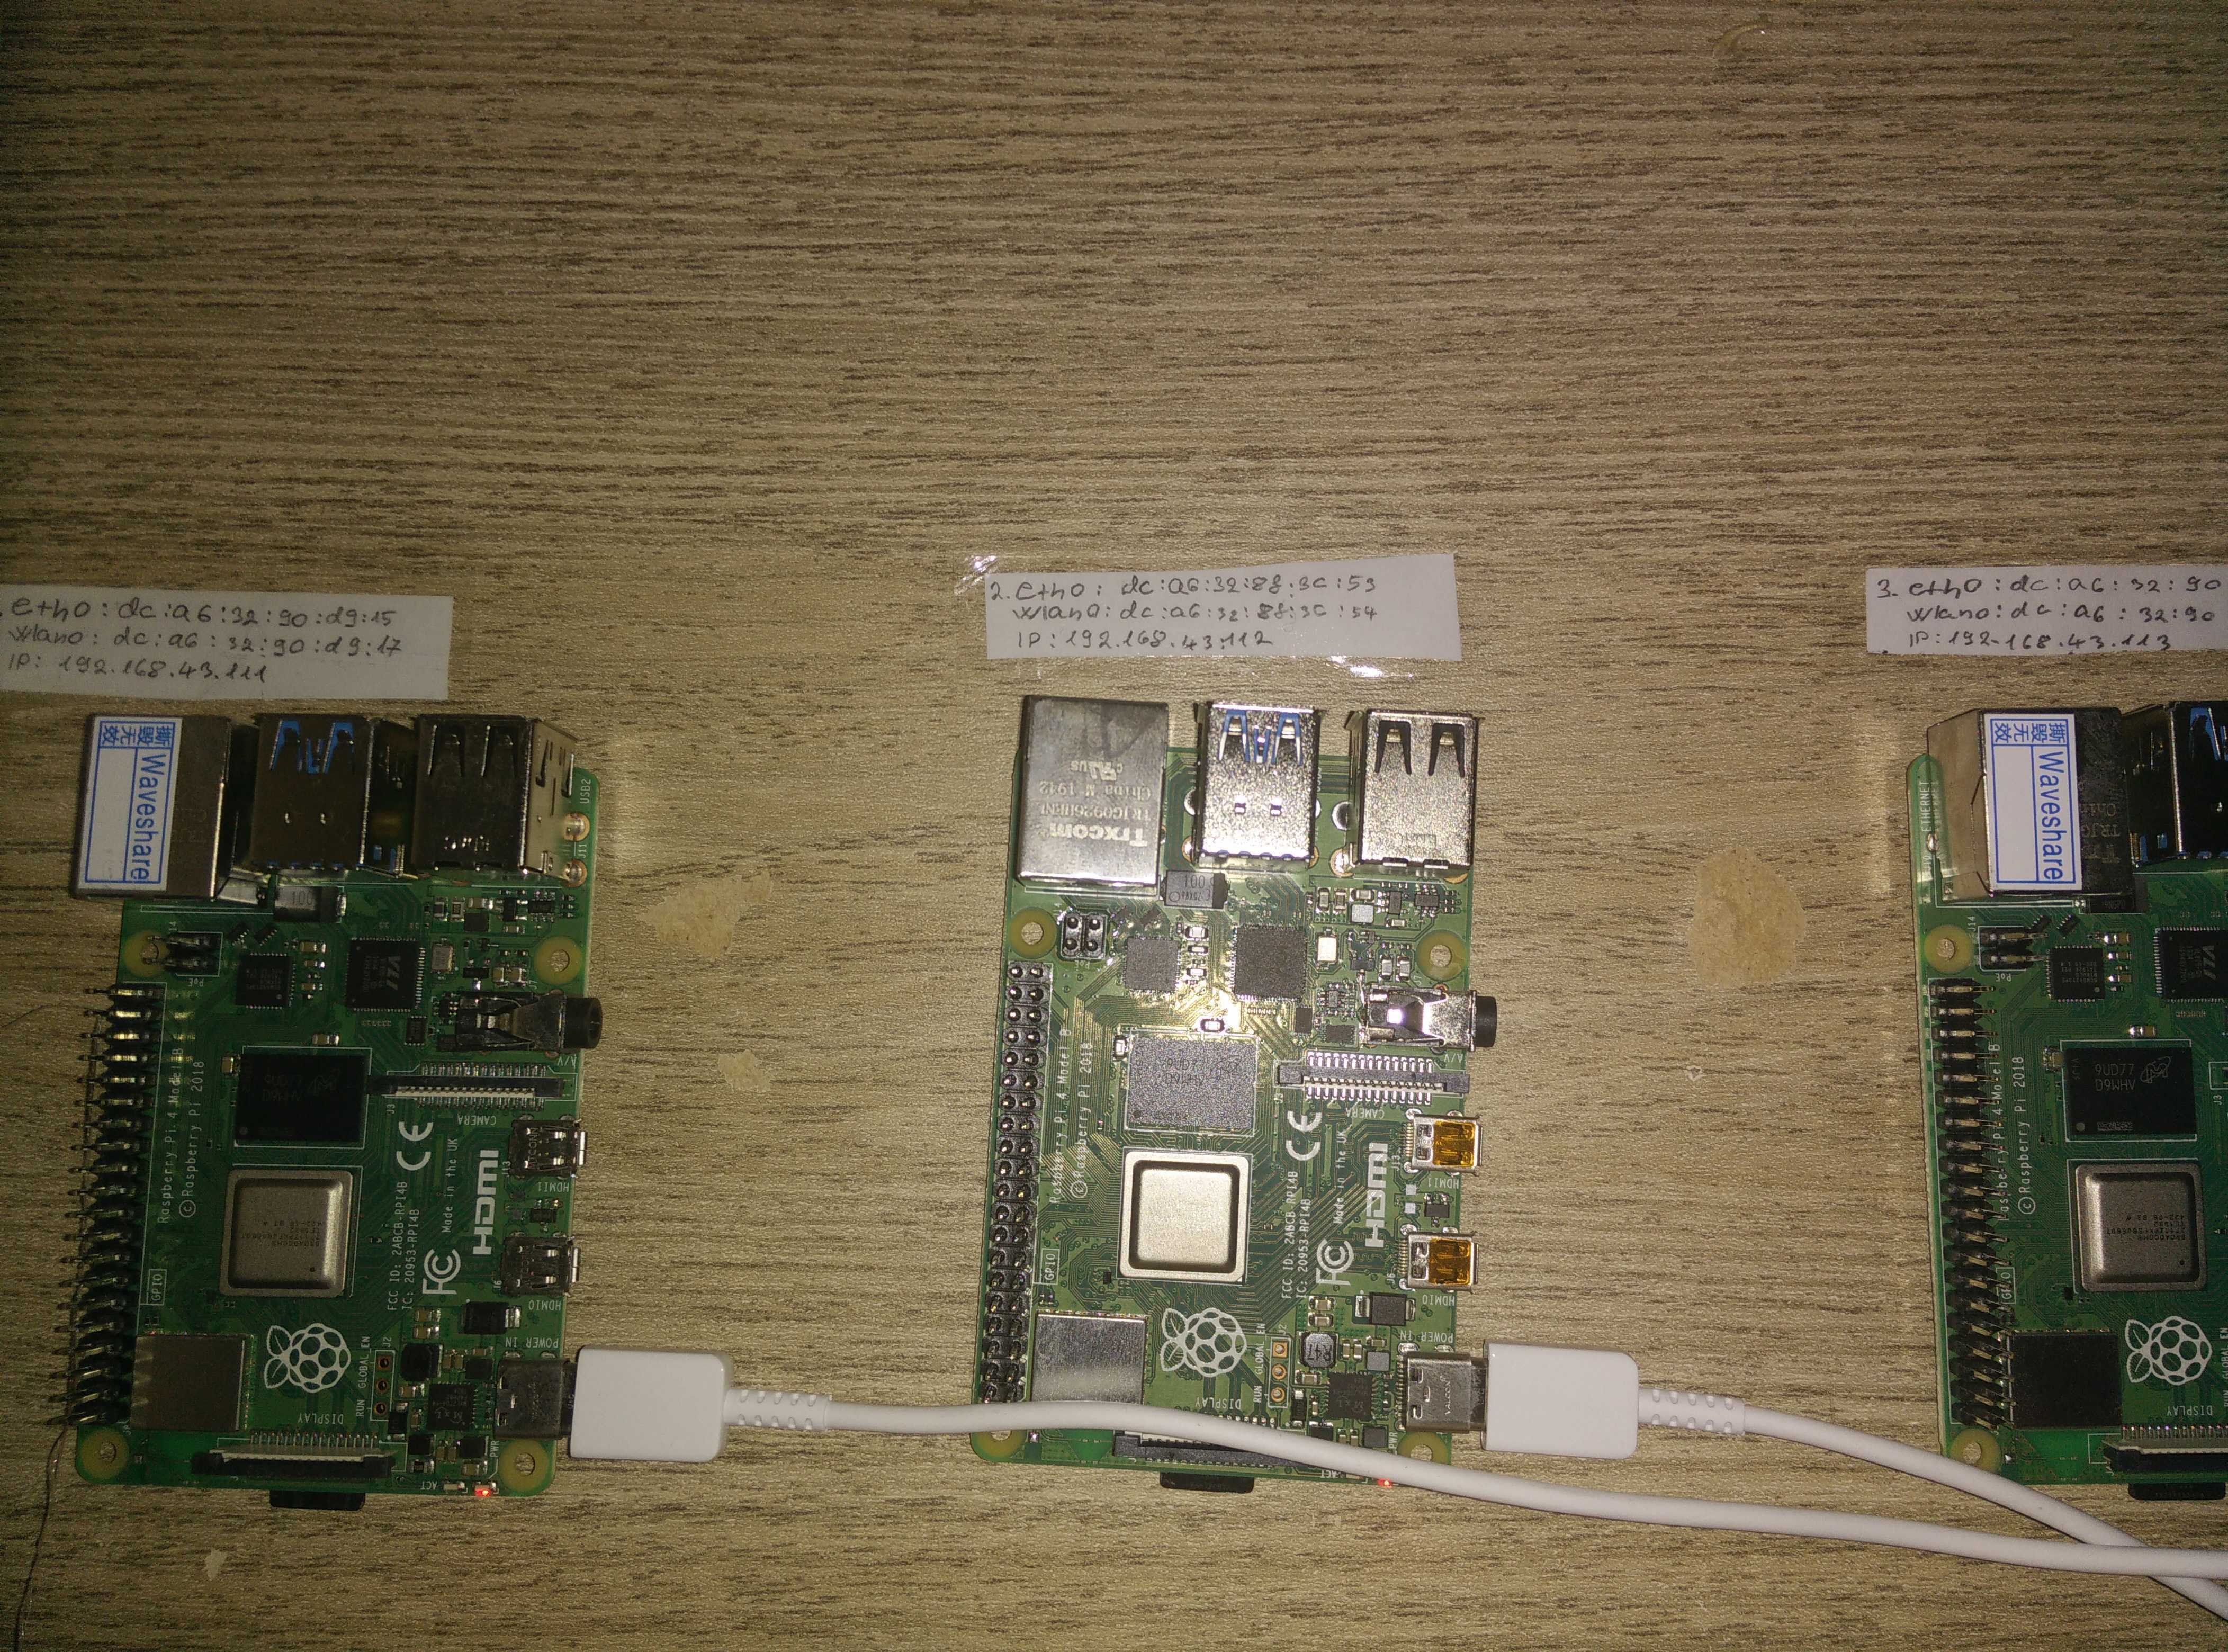
\includegraphics[width=1.0\textwidth]{images/postavitev-raspberry.jpg}
\end{center}
\caption{Postavitev gruč Raspberry PI.}
\label{rpi-gruce}
\end{figure}
\section{K3S in K3OS}
Obstaja več implementacij Kubernetesa.
Mi bomo uporabili z viri varčno odprtokodno implementacijo K3S od podjetja Rancher~\cite{k3s-info}~\cite{k8s-performance-comparison}~\cite{low-resource-k8s}.
Hkrati so v podjetju Rancher pripravili distribucijo operacijskega sistema Linux K3OS~\cite{k3os-git}.
Gre za minimalen operacijski sistem s prednameščenim sistemom K3S.
Te\-ža\-va se pojavi, ker uradna verzija operacijskega sistema za ploščice Raspberry PI še ni pripravljena.
K sreči pa se je v ta namen začel odprtokodni projekt \emph{PiCl k3os image generator}, ki iz slik operacijskih sistemov K3OS in Raspberry OS ter konfiguracijskih datotek zgradi novo sliko operacijskega sistema za naš Raspberry PI ~\cite{k3os-rpi-image-generator}.
Konfiguracijske datoteke, ki jih moramo priložiti so standardne datoteke YAML, ki jih podpira sistem K3OS.
Vanje zapišemo nastavitve kot so javni ključi za dostop SSH, podatki omrežja Wi-Fi na katerega se povezujemo, geslo, žeton za povezavo z gručo Kubernetes in način, v katerem želimo zagnati K3S na sistemu~\cite{k3os-git}.
\begin{figure}[h]
  \begin{verbatim}
ssh_authorized_keys:
- ssh-rsa ...
hostname: gruca-1
k3os:
  ntp_servers:
  - ...
  password: ...
  token: ...
  dns_nameservers:
  - ... 
  wifi:
  - name: ...
    passphrase: ...
  k3s_args:
  - server
\end{verbatim}
\end{figure}

V našem primeru smo vse programe K3S zagnali v strežniškem načinu (server) in nobenega v načinu delovnega vozlišča, saj želimo, da vsak Raspberry PI predstavlja svojo gručo.
\section{Demonstracijska spletna aplikacija}
Za potrebe testiranja je bilo treba narediti novo testno storitev.
Ker se želimo v tem diplomskem delu osredotočiti na realne probleme, s katerimi se srečujejo podjetja, mora ta aplikacija omogočati tudi shranjevanje podatkov v podatkovno bazo.

Koda, ki je javno objavljena v repozitoriju Git~\cite{git-stateful-rest-sample}, je napisana v programskem jeziku Go.
Iz kode je bil generiran kontejner, ki je objavljen v javnem registru Docker~\cite{docker-stateful-rest-sample}.
Ob tem velja opozoriti, da Raspberry PI uporablja arhitekturo procesorja ARM, kar je zahtevalo dodatno pozornost pri nastavitvah gradnje ustrezne slike Docker.

Aplikacija na mrežnih vratih, podanih s spremenljivko okolja, izpostavi vmesnik REST, ki podpira dva preprosta HTTP klica.
\spverb|GET| klic na pot \spverb|/users| nam bo vrnil seznam vseh uporabnikov, ki so zapisani v tabeli v podatkovni bazi, s klicem \spverb|POST| na isto pot pa poskrbimo, da se podatki uporabnika iz našega zahtevka shranijo v tabelo v podatkovni bazi.
\begin{verbatim}
# ukaz za dodajanje uporabnika
curl -X POST localhost/users \
  --data '{"name": "John", "lastname": "Doe"}'
# ukaz za prikaz vseh uporabnikov
curl localhost/users
\end{verbatim}

Za shranjevanje podatkov bomo uporabili dve različni bazi podatkov SQL: Postgres, ki je preprosta za lokalni razvoj, a ne omogoča napredne sinhronizacije podatkov med strežniki in CrateDB, ki je bil zasnovan kot baza SQL na več vozliščih in nam omogoča napredne sinhronizacije tudi med različnimi strežniki in gručami.
K sreči pa CrateDB implementira vmesnik PostgreSQL in nam kode za prehod med bazami ni potrebno spreminjati~\cite{cratedb}.
\section{Namestitev KubeFed}
Kot ena izmed ključnih komponent složnega delovanja več gruč je njihovo upravljanje.
V te namene bomo uporabili program KubeFed, ki ga moramo namestiti na eno izmed gruč, ki jih želimo povezati skupaj.
Ker je izdelek še v razvoju in še ni prišel iz alfa faze, še ni objavljene uradne verzije programa za arhitekturo ARM.
Zato je bilo iz kode KubeFed treba zgraditi novo sliko kontejnerja, ki je javno objavljena~\cite{docker-kubefed}.
Potem pa smo uporabili uradno predlogo Helm, pri čemer smo samo zamenjali originalno sliko kontejnerja z našo.
Za delo s KubeFed pa moramo na svoj računalnik namestiti še orodje kubefedctl.
Z uporabo ukaza \spverb|kubefedctl join| povežemo vse tri gruče v sistem KubeFed.
\begin{verbatim}
kubefedctl join gruca-1
kubefedctl join gruca-2
kubefedctl join gruca-3
\end{verbatim}
S tem smo uspešno povezali več gruč Kubernetes v sistem KubeFed.
Seznam vseh povezanih gruč pa lahko preverimo tako, da izpišemo seznam objektov tipa KubeFedClusters. 
V našem primeru imamo povezane tri gruče, kar se vidi iz sledečega izpisa.
\begin{verbatim}
kubectl get kubefedclusters

NAME        AGE   READY
gruca-1     1d    True
gruca-2     1d    True
gruca-3     1d    True
\end{verbatim}
Sedaj lahko z uporabo ukazov \spverb|kubefedctl enable| in \spverb|kubefedctl federate| naše objekte dodajamo v vse gruče hkrati.

\chapter{Povezovanje med podatkovnimi centri}
\label{povezovanje-med-centri}
\section{Problem velike latence}
Za primer vzemimo preprosto spletno aplikacijo, ki mora hraniti stanje in jo namestimo v eno gručo Kubernetes.
Če to aplikacijo ponudimo vsem uporabnikom na globalnem trgu, se nam bo pojavil problem velike latence~\cite{minimizing-latency}.
To pomeni, da bo naša aplikacija za uporabnike, ki so bolj oddaljeni od naše gruče, delovala počasneje oziroma se bodo ob enaki pasovni širini podatki do uporabnika prenašali dalj časa.

Takšen problem v splošnem rešimo tako, da našo aplikacijo postavimo še v dodatno gručo, bližje uporabniku~\cite{geo-instability}.
Če moramo podatke med gručami še sinhronizirati, pa to zahteva dodaten trud.
V našem primeru bomo uporabili podatkovno bazo CrateDB~\cite{cratedb}, novejšo alternativo standardnim podatkovnim bazam SQL.
CrateDB ima v primerjavi s tradicionalnimi podatkovnimi bazami boljšo podporo za sinhronizacijo podatkov med vozlišči ~\cite{databases-comparison}.
Poleg vsega pa nam za uporabo podatkovne baze CrateDB ni treba konceptualno spreminjati naše aplikacije, saj podpira vmesnik podatkovne baze PostgreSQL.
\section{Povečanje razpoložljivosti aplikacije}
Če je čim višja razpoložljivost za našo aplikacijo kritičnega pomena in smo že poskrbeli za visoko razpoložljivost (HA) aplikacije v naši gruči, še vedno lahko pride do situacije, ko iz omrežja izpade ves podatkovni center~\cite{cloud-failures}.
Spomnimo se, da Kubernetes najbolj učinkovito deluje, če naša vozlišča uporabljajo hitro notranje omrežje podatkovnega centra.
V primeru napake v podatkovnem centru ali hujših vremenskih pogojev, ki bi prekinili povezave do podatkovnega centra, to pomeni, da je nedosegljiv ves podatkovni center in s tem gruča v njem.
Pri uporabi strežnikov v oblaku lahko še povečamo razpoložljivost tako, da gruče namestimo v različne razpoložljivostne cone (availability zones) in podatkovne centre pri enem ali celo več različnih oblačnih ponudnikih.
Takšen pristop je opisan v članku~\cite{tosca-fed}, omogoča pa ga predvsem neodvisnost Kubernetesa od platform.
\section{Povezovanje med podatkovnimi centri}
Rešitev za oba omenjena problema je enaka.
Postaviti moramo gruče v več različnih podatkovnih centrih in jih nastaviti, da bodo delovale usklajeno.
Ti podatkovni centri bodo bližje uporabniku ali pa v lasti različnih oblačnih ponudnikov -- odvisno od problema.
  Princip pa ostaja.
\section{Razporeditev uporabnikov po gručah}
Ko imamo na vsaki gruči javno izpostavljen Kubernetesov objekt Service in postavljene primerne objekte Ingress, moramo uporabnike še vedno usmeriti na njim najbližjo gručo.
Lahko jih usmerimo avtomatsko z zapisi DNS, ki omogočajo usmerjanje na podlagi geolokacije.
Lahko uporabimo in namestimo zunanji DNS skozi Kubernetes ali pa to opravimo kar mimo Kubernetesa.
V naših lokalnih testnih gručah bomo ta korak preskočili in uporabnikov ne bomo usmerjali preko javnih strežnikov DNS, saj v lokalnem okolju to ni smiselno.
\begin{figure}[h]
\begin{center}
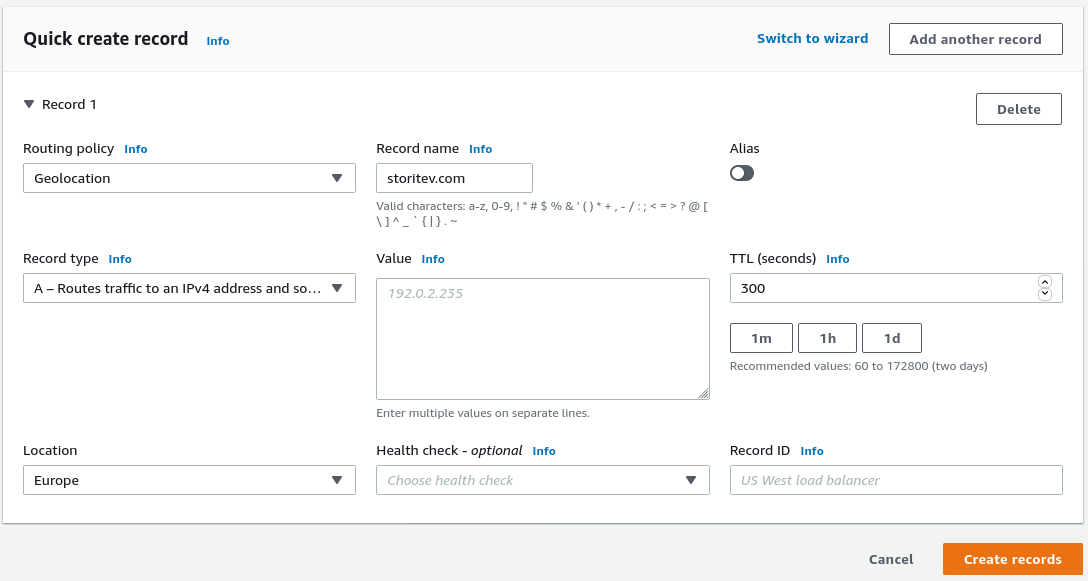
\includegraphics[width=1.0\textwidth]{images/geolokacijski-dns.png}
\end{center}
  \caption{Ustvarjanje geolokacijskega zapisa DNS v storitvi Route53.}
\label{primer-ustvarjanje-geolokacijskega-zapisa}
\end{figure}

Naslednja možnost je rešitev, ki se je poslužujejo nekatere internetne računalniške igre (npr. Among Us), in sicer, da so naši strežniki popolnoma ločeni in se vsak uporabnik sam odloči, na kateri gruči ali strežniku želi igrati.
V takšnih primerih se lahko izognemo problemu sinhronizacije podatkov med strežniki, kar zelo poenostavi upravljanje naših gruč.
\section{Definicija infrastrukture za naš primer}
V našem primeru spletne aplikacije bomo imeli v vsaki gruči eno postavitev aplikacije \emph{Stateful rest sample} z objektom Deployment. 
Da aplikacijo izpostavimo izven gruče, pa bomo uporabili objekt Service.
Aplikacija bo za shranjevanje uporabljala podatkovno bazo CrateDB, ki bo postavljena z objektom statefulSet, diskom na lokalni kartici SD, in dvema objektoma Service.
Prvi objekt Service je zunanji in se bo uporabljal za dostop do baze, drugi pa je notranji in ga bomo uporabljali za prepoznavo ostalih primerkov CrateDB v gruči.
\begin{figure}[h]
\begin{center}
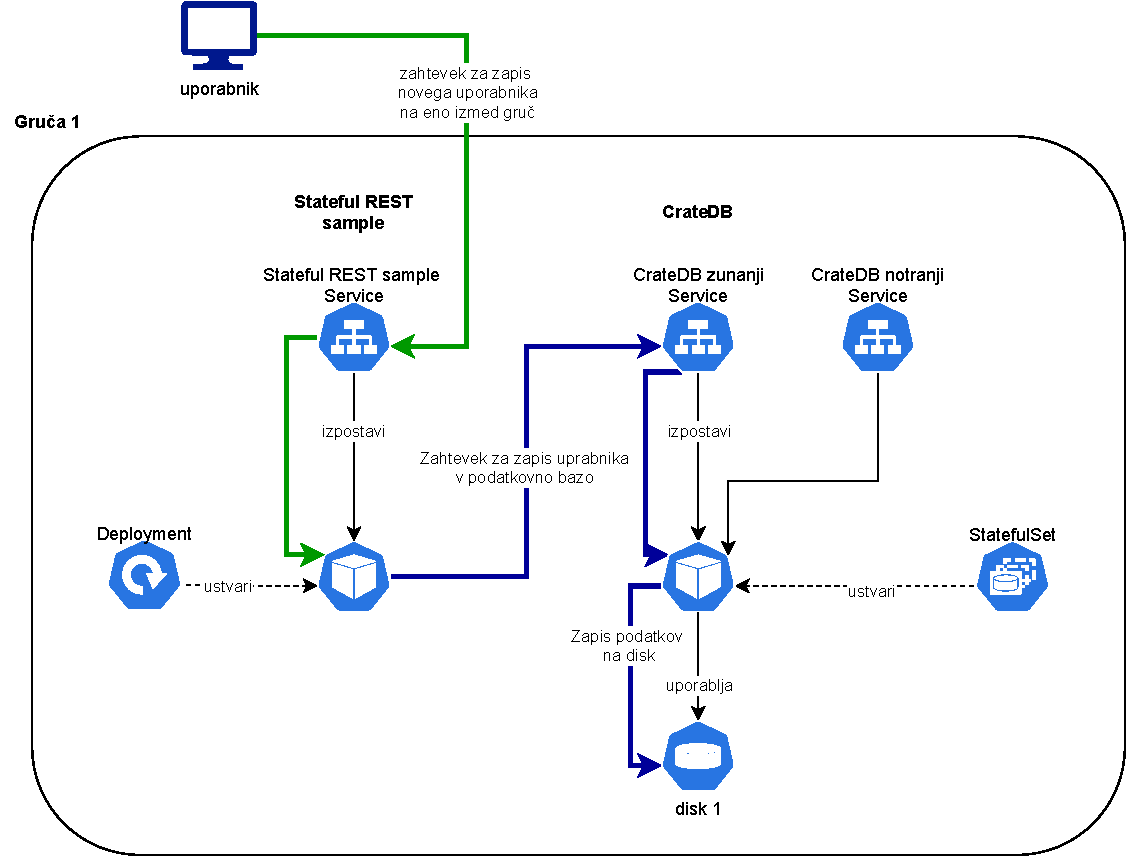
\includegraphics[width=1.0\textwidth]{images/infrastructure-example.pdf}
\end{center}
\caption{Infrastruktura vsake gruče v primeru demonstracijske aplikacije}
\label{infrastructure-example}
\end{figure}
Vsa konfiguracija je javno objavljena na repozitoriju Git\cite{git-diploma}.
Postavimo jo z ukazom \spverb|kubectl apply -f diploma-demo-1|.
Takoj preverimo, če aplikacija deluje in če lahko podatke zapisujemo v bazo.
To storimo tako, da prek demonstracijske aplikacije poskusimo dodati uporabnika in izpisati vse uporabnike.
To naredimo z naslednjima ukazoma \spverb|curl|.
\begin{verbatim}
curl -X POST gruca-1/users \
    --data '{"name": "John", "lastname": "Doe"}'
curl gruca-1/users
\end{verbatim}
\section{Implementacija s KubeFed}
Najprej se moramo odločiti, za katere tipe objektov bomo vklopili federacijo oziroma za katere bomo želeli univerzalno upravljanje.
V našem primeru gre za Service, Deployment in StatefulSet.
Vklopimo jih z naslednjim ukazom, ki za nas ustvari nove federirane tipe objektov na izbranih tipih.
\begin{verbatim}
kubefedctl enable <ime tipa>
\end{verbatim}
Ko vklopimo federacijo na vseh potrebnih tipih, pa moramo vklopiti še avtomatsko upravljanje na specifičnih objektih.
V našem primeru želimo za to uporabiti ukaz \spverb|kubefedctl federate|.
\begin{verbatim}
kubefedctl federate deployment stateful-rest-sample
kubefedctl federate service stateful-rest-sample
kubefedctl federate statefulset crate
kubefedctl federate service crate-internal
kubefedctl federate service crate-external
\end{verbatim}
Izvršeni ukazi ustvarijo federirane objekte, ki uporabijo postavitev v vse gruče in za predlogo kar podane objekte.
Tako je za nas rezultat izvršenih ukazov kreiranje federiranih objektov in posledično kopiranje objektov v vse naše povezane gruče.

Po preizkusu delovanja z ukazom \spverb|curl| opazimo, da podatki med gručami še vedno niso sinhronizirani.
Uporabniki, ki jih vnesemo v eno gručo, se še ne sinhronizirajo v ozadju.
Na tej točki se ustavijo nekatere spletne aplikacije in prepustijo izbiro strežnika oziroma gruče kar uporabniku.
\section{Sinhronizacija podatkov}
Če želimo pred uporabnikom skriti, da uporabljamo več gruč, moramo poleg geolokacijskih zapisov DNS urediti tudi avtomatsko sinhronizacijo podatkov.
V našem primeru res uporabljamo samo en primerek baze CrateDB na gručo, a vseeno smo na nivoju sinhronizacije znotraj gruče to že uredili. 
Moramo se zavedati, da tudi podatkovna gruča CrateDB najbolje deluje, če so vozlišča v hitrem lokalnem omrežju z visoko pasovno širino in nizko latenco.
CrateDB podpira tudi sinhronizacijo med različnimi razpoložljivostnimi conami in podatkovnimi centri~\cite{cratedb-zone}.
\subsection{Uporaba primerne podatkovne baze}
Za sinhronizacijo podatkov lahko uporabimo podatkovno bazo, ki ima sinhronizacijo med različnimi gručami že podprto.
CrateDB podpira sinhronizacijo tudi preko razpoložljivostnih con.
Vseeno pa moramo vsa vozlišča povezati v enako podatkovno gručo~\cite{cratedb-zone}.
To pomeni, da morajo biti primerki CrateDB dostopni med seboj.
Problem lahko rešimo z uporabo sistema Cilium in uporabo globalnih storitev, saj nam Cilium že omogoča komunikacijo vsakega kontejnerja z vsakim, tudi če so ti v različnih gručah.
Druga možnost pa je, da izpostavimo vsak objekt Pod s svojim javnim naslovom IP in jih v gručo povežemo ročno.

Določiti moramo še nastavitve za zmanjšanje prometa med podatkovnimi centri in nastavitve za zagotavljanje prisotnosti podatkov v vsakem podatkovnem centru~\cite{cratedb-zone}.
Podobne načine sinhronizacije podpira tudi na primer podatkovna baza Cassandra~\cite{cassandra-zone}.
\subsection{Ročno usklajevanje podatkov}
Sinhronizacija podatkovne baze ni trivialen problem.
Če ne uporabimo primerne podatkovne baze ali pa preko gruč želimo sinhronizirati samo del podatkov, bomo sinhronizacijo podatkov verjetno morali implementirati sami.
To pomeni, da bomo ustvarili novo storitev, ki bo v ozadju kopirala ključne podatke med podatkovnimi centri.
Ker samo mi poznamo naš konkreten primer uporabe, je takšen pristop lahko najbolj učinkovit, a tudi najbolj kompleksen in časovno potraten.

V našem primeru bomo s preprosto skripto kopirali uporabnike iz ene aplikacije v drugo kar z uporabo vmesnika REST.
To bomo storili v drugem kontejnerju Ubuntu z uporabo ukazov \spverb|curl| za izvajanje klicev REST in ukazom \spverb|jq|~\cite{jq} za razčlenjevanje podatkov.
Podatki se sinhronizirajo vsakih deset sekund.
Primer še testiramo in dobimo spodnji izhod, kar potrdi, da so se podatki uspešno sinhronizirali.
\begin{verbatim}
curl -s -X POST gruca-1/users \
  --data '{"name": "John", "lastname": "Doe"}'
curl -s gruca-2/users
[{"Name":"John","Lastname":"Doe"}]
\end{verbatim}
\chapter{Upravljanje izoliranih aplikacij}
\section{Zmanjševanje posledic vdorov in izpadov}
Računalniška stroka si je že nekaj časa nazaj priznala, da popolnega sistema ne more ustvariti: sistema, ki se ne more sesuti, sistema, ki bo ves čas razpoložljiv, in sistema, v katerega ne bo mogoče vdreti.
To vsake toliko časa potrdijo tudi najbolje upravljani veliki sistemi, kot so AWS, Google, Facebook z izpadi ali vdori na njihovih storitvah~\cite{common-outages}. 
Vseeno pa lahko kljub vdorom in napakam, zaradi katerih postanejo naši sistemi nedosegljivi, vedno poskusimo zmanjšati posledice ob morebitnem vdoru ali izpadu. 
\subsection{Izpadi aplikacije}
Kljub temu, da smo naše aplikacije namestili na različne gruče, s čimer je aplikacija odporna na izpad ene gruče, pa lahko ob hujših nepravilnostih delovanja ene aplikacije in napaki pri nastavitvi gruč kaskadno izpadejo tudi vse gruče, na katerih imamo aplikacijo nameščeno.
Takšen primer je, ko ena aplikacija ali storitev zavzame vse vire v gruči, hkrati pa odpovejo ostale varovalke, ki jih ponuja že sam Kubernetes.
V takšnih primerih bo namesto samo dela odpovedal celoten sistem.
Zato se lahko odločimo, da bomo nekatere bolj kritične aplikacije ali storitve postavili v ločeno gručo, kjer napake drugih aplikacij ne bodo vplivale na delovanje kritičnih.
A vseeno se moramo zavedati, da je ta korak smiseln šele po tem, ko opravimo že vse predhodne preventivne ukrepe, kot so razdelitev aplikacije na mikrostoritve, kontejnerizacija, pravilna nastavitev omejitev skaliranja aplikacije in druge.
\subsection{Vdori}
Podobno kot pri izpadih aplikacije je tudi pri preprečevanju posledic vdorov.
Najprej moramo poskrbeti za primerno zaščito vozlišč Kubernetes, naše aplikacije, zaščito komunikacije med storitvami, uporabo nepriviligiranih kontejnerjev~\cite{securing-kube}.
Če pa nam vsi zgoraj našteti in ostali priporočeni ukrepi niso dovolj, ali pa se zavedamo, da imamo v gručah manj varne aplikacije in napadalec prek njih ne sme dostopati do podatkov kritičnih aplikacij, potem je smiselno kritične aplikacije izolirati v svoje gruče.
\section{Implementacija s KubeFed}
\begin{figure}[h]
\begin{center}
  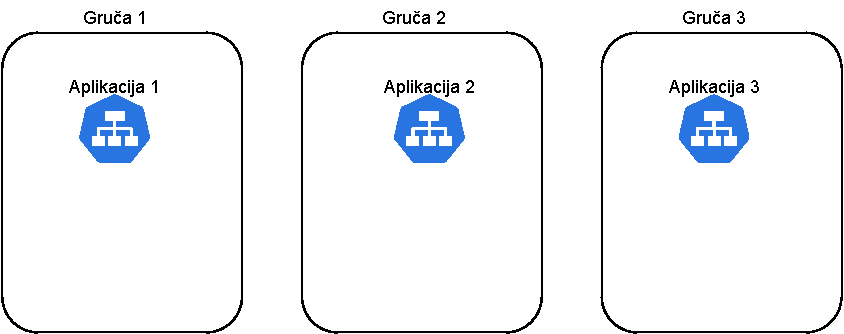
\includegraphics[width=1.0\textwidth]{images/primer-izolirane-aplikacije.pdf}
\end{center}
\caption{Primer izoliranih aplikacij.}
\label{problem-prevelike-latence}
\end{figure}
Ena izmed treh glavnih lastnost federiranih objektov je možnost izbire gruč, na katerih se bo določen objekt ustvaril. 
S tega stališča je naš primer zelo preprost.
Samo določimo, da se naša aplikacija izvaja na gruči 3 namesto na vseh.
Tokrat za federacijo ne moremo uporabiti ukaza \spverb|kubefedctl federate|, ampak moramo konfiguracijo federiranih objektov spisati sami.
Najprej bomo z ukazom \spverb|kubectl tag| označili našo izolirano gručo (ali več njih).
Potem pa bomo lastnosti \spverb|.clusterSelector.matchLabels| vsakega federiranega objekta, ki ga želimo izolirati, dodali označbe vseh izoliranih gruč.
V takšnih primerih se nam ni treba posebej ukvarjati s sinhronizacijo podatkov, saj smo vse podatke obdržali v isti gruči ali pa sinhronizirali na enak način kot v poglavju \ref{povezovanje-med-centri}.
\chapter{Upravljanje gruč na robu oblaka}
\label{edge-clusters}
\section{Gruče na robu oblaka}
Razlogov, zakaj gruče postavljamo na rob oblaka oziroma fizično bližje konč\-ne\-mu uporabniku, je več.
Za primer vzemimo zahtevo podjetja, da se morajo njihovi podatki obdelovati lokalno -- v njihovem podjetju.
V našem primeru se bomo osredotočili na upravljanje takšnih gruč.
\section{Implementacija s KubeFed}
Ko enkrat povežemo vse gruče z ukazom \spverb|kubefedctl join|, je njihovo upravljanje preprosto.
Samo nastavimo v kateri gruči želimo katere objekte, in naša naloga je končana.
Zavedati se moramo, da nekaj prenosa podatkov porabi tudi KubeFed za sinhronizacijo, zato moramo biti pozorni, če se podatki prenašajo prek dragih mobilnih omrežij.
\begin{figure}[h]
\begin{center}
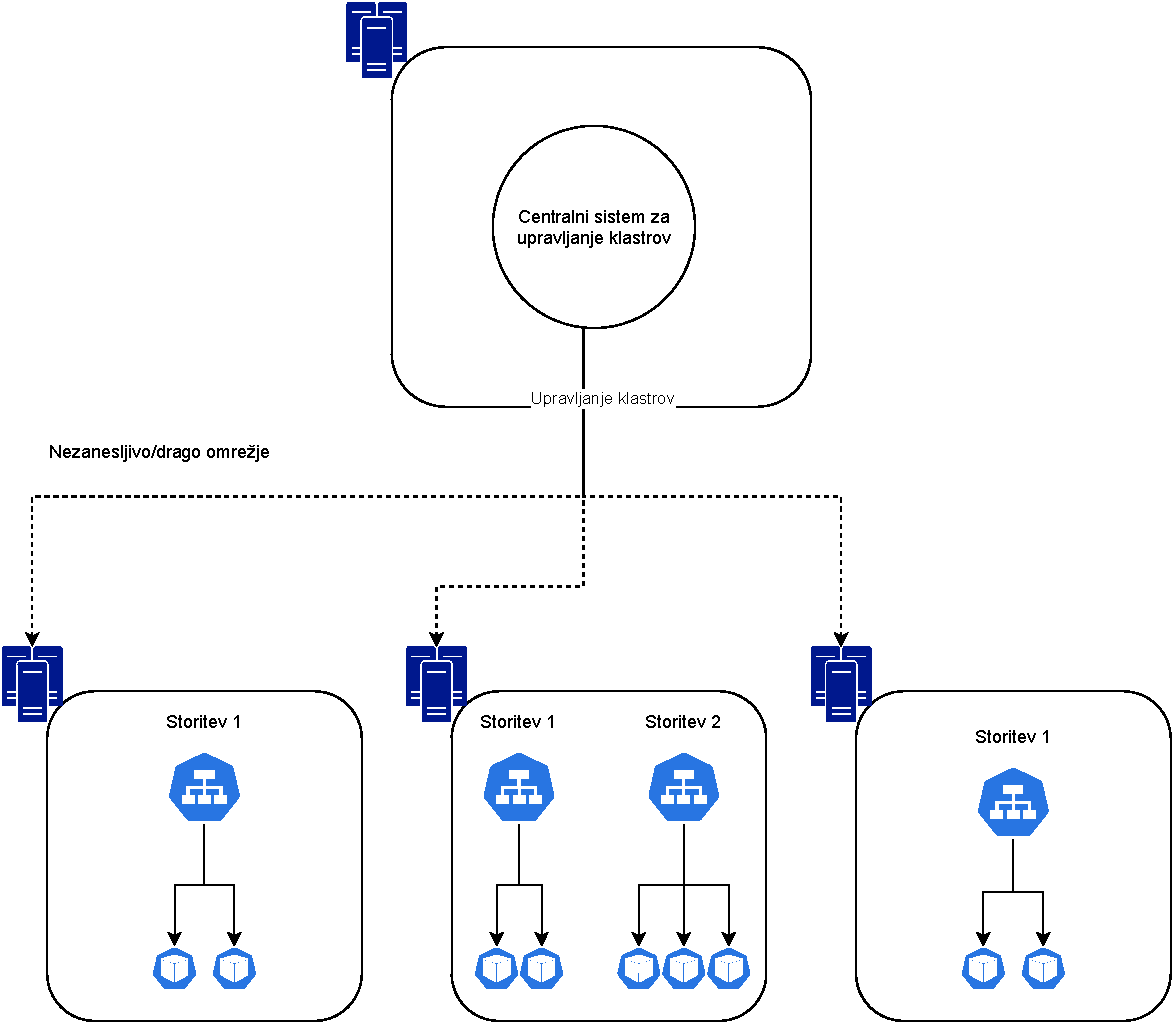
\includegraphics[width=1.0\textwidth]{images/upravljanje-robnih-gruc.pdf}
\end{center}
\caption{Primer upravljanja gruč na robu oblaka.}
\label{problem-prevelike-latence}
\end{figure}

Nam pa KubeFed omogoča še eno možnost s svojo strukturo.
S svojim kontrolerjem in vmesnikom KubeFed lahko implementiramo še dodatne funkcionalnosti, kot so razporejanje obremenjenosti med lokalnimi strežniki, in po potrebi povečujemo število primerkov, ali pa kar razporejamo opravila z objekti Kubernetes Job.

Z zelo preprosto integracijo v sistem Kubernetes nam vmesnik KubeFed tu omogoča zelo preprosto implementacijo katerekoli naše rešitve.
\section{Sinhronizacija podatkov}
V primeru gruč na robu oblaka bomo sinhronizacijo verjetno implementirali sami, saj le mi vemo, kakšen problem rešujemo in zakaj smo sploh postavljali gruče na robu oblaka.

Za primer vzemimo hipotetični varnostni sistem korporacije, ki centralno spremlja varnost v posameznih podružnicah.
Sistem ima eno nadzorno kamero pri vhodu v vsako podružnico.
Želimo, da naša kamera prepoznava obraze in na podlagi tega zaposlenim dovoljuje vstop.
V našem centralnem sistemu pa želimo hraniti seznam vstopov.
En način reševanja tega problema je z gručami na robu oblaka.
V vsako podružnico bi postavili gručo rač\-un\-al\-ni\-kov Raspberry PI, ki so dovolj zmogljivi, da obdelujejo posnetke kamer in prepoznavajo obraze.
Če posnetke obdelujemo lokalno, se izognemo pošiljanju velike količine podatkov na centralne strežnike, posledično pa bo hitrejše tudi preverjanje zaposlenih.
Tako bi na centralni strežnik pošiljali samo številko zaposlenega in čas vstopa.
Takšen pristop bi prišel še toliko bolj do izraza, če imajo podružnice dostop do interneta samo prek dragega mobilnega omrežja, kjer lahko z zmanjšanjem prometa zelo zmanjšamo stroške podjetja.
Vse te gruče na podružnicah bi imele zelo podobno strukturo in jih je smiselno centralo upravljati z nekakšnim sistemom za povezovanje. 
Tu bi lahko uporabili pristopa KubeFed ali pristop GitOps.
Pošiljanje podatkov v centralno gručo pa bi morali implementirati sami in ga vgraditi v naš program za prepoznavo obrazov.
\chapter{Sklepne ugotovitve}
V diplomskem delu smo predstavili teoretično ozadje povezovanja več rač\-un\-al\-ni\-ških gruč Kubernetes.
Predstavljenih je bilo tudi nekaj popularnih orodij za delo z njimi.
V praktičnem delu smo se posvetili predvsem reševanju pogostih problemov, s katerimi se srečujejo podjetja v praksi, ki zahtevajo povezovanje več gruč.
Razvili smo primer preproste aplikacije za shranjevanje uporabnikov, s pomočjo katere smo reševali problem povezovanja več gruč Kubernetes.
Pokazali smo, da je ob uporabi primernih orodij upravljanje več gruč Kubernetes preprosto, bolj zahtevna pa je sinhronizacija podatkov med različnimi gručami, kar smo pokazali tudi na primeru.
Če je možno, se je sinhronizaciji podatkov smiselno izogniti.
Takšen pristop smo uporabili tudi v podjetju, kjer sem zaposlen.

Z razvojem Kubernetesa se je razvilo tudi zelo veliko odprtokodnih orodij, ki omogočajo lažje upravljanje in povezovanje več gruč.
Tako so napredne tehnologije prišle v roke širšemu krogu ljudi in jim omogočajo preprostejše reševanje problemov.
Kubernetes pa je s standardizacijo orkestracije zelo olajšal tudi možnost gostovanja aplikacije pri več različnih oblačnih ponudnikih, kjer se zopet pojavi problem povezovanja več gruč.

Področje orkestracije in povezovanja gruč se bo še zelo razvijalo.

\newpage %dodaj po potrebi, da bo številka strani za Literaturo v Kazalu pravilna!
\newpage %dodaj po potrebi, da bo številka strani za Literaturo v Kazalu pravilna!
\newpage %dodaj po potrebi, da bo številka strani za Literaturo v Kazalu pravilna!
\newpage %dodaj po potrebi, da bo številka strani za Literaturo v Kazalu pravilna!
\ \\
\clearpage
\addcontentsline{toc}{chapter}{Literatura}
\bibliographystyle{plain}
\bibliography{literatura}
\end{document}
